\begin{itemize}
    \item K-means  uses Euclidean Distance, uses Mean as representative: Centroid
    \item K-means  has a parameter K that you need to guess before clustering (Choice of K is crucial, may stuck at local minimum)
    \item \textbf{Failure in case of non spherical data but FAST !}
    \item Iterative two-step approach?  1- Cluster Assignment,  2- Centroid Update\\When to stop?  1- No update in the assignment  , 2- Max iterations reached
    \item \textbf{Randomness of K-means}: Centroids are chosen first at random , May not find the same solution every time. Then, run several times, and the run with the lowest SSE value is chosen to report the final clustering.
    \begin{figure}[H]
        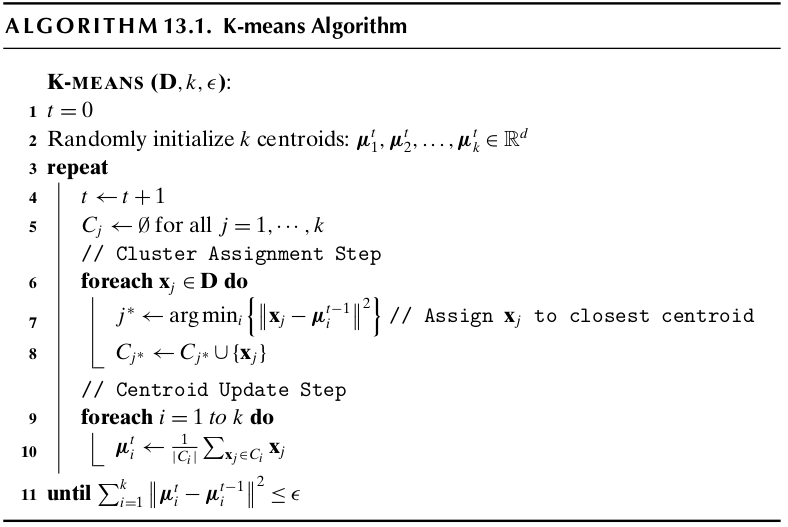
\includegraphics[width=0.8\textwidth]{Figures/kmeans.png}
        \caption{\label{fig:figure3}K-Means Algorithm, total time is O(tknd).}
    \end{figure}
\end{itemize}